\chapter{功能安全和信息安全性质}

\section{Safety Property}
Safety Property描述了协议的功能安全性质,在使用sbid工具进行协议建模时,用于对模型进行安全性质规约,用于模型检测的过程中发现伪反例后,通过归纳不变式去除伪反例,从而对模型进行精化。在[协议>概览>类图]下,点击小工具栏上的[创建Safety Property]按钮,即可创建新的Safety Property的类图,如图\ref{create_safety}所示。
\begin{figure}[h]
	\centering
	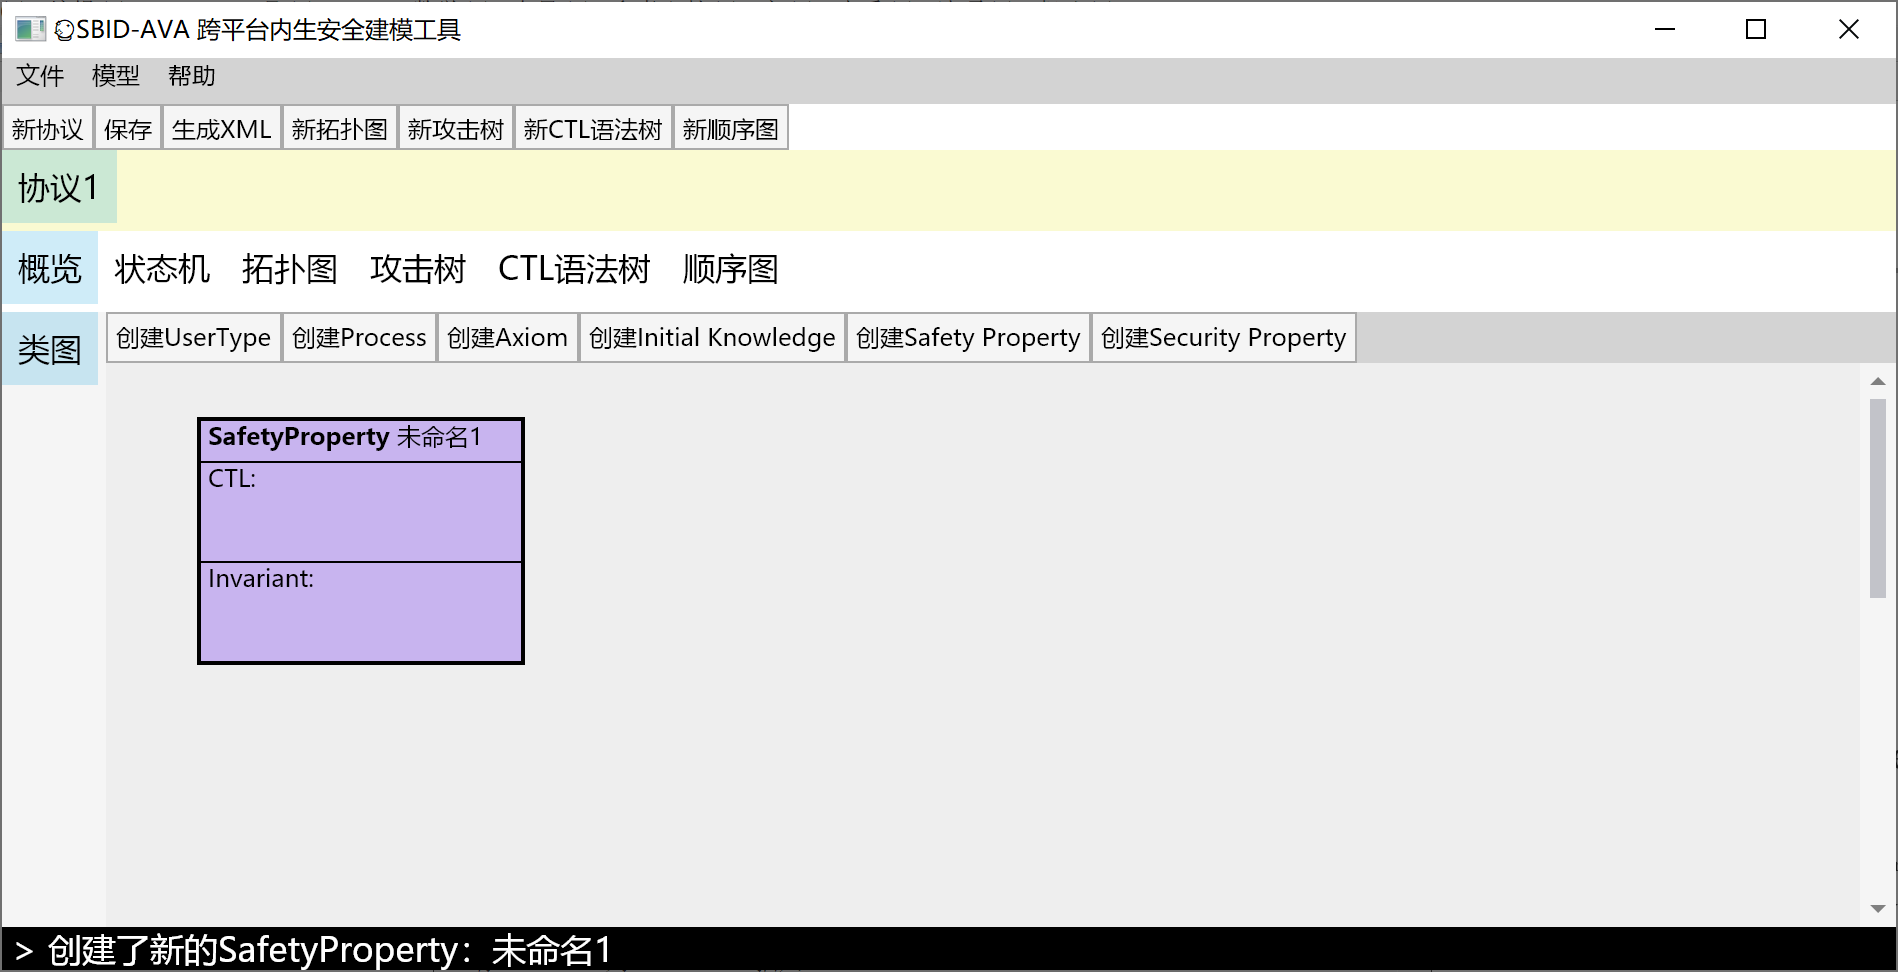
\includegraphics[width=12cm,height=6.75cm]{imgs/create_safety.png}
	\caption{新创建的Safety Property}
	\label{create_safety}
\end{figure}
\par
在sbid工具中,支持用户对Invariants(不变性)和CTL(Computation Tree Logic)进行描述。
\par
在Safety Property的类图上右键,呼出右键菜单,点击[编辑],即可打开在Safety Property的编辑窗体。
\subsection{Invariant}
\par
Safety Property的Invariant用于定义模型的不变性条件。在Safety Property的编辑窗口选择[Invariant]选项卡,可对不变性条件进行添加、修改和删除,如图\ref{safety_edit_invariants}所示。
\begin{figure}[h]
	\centering
	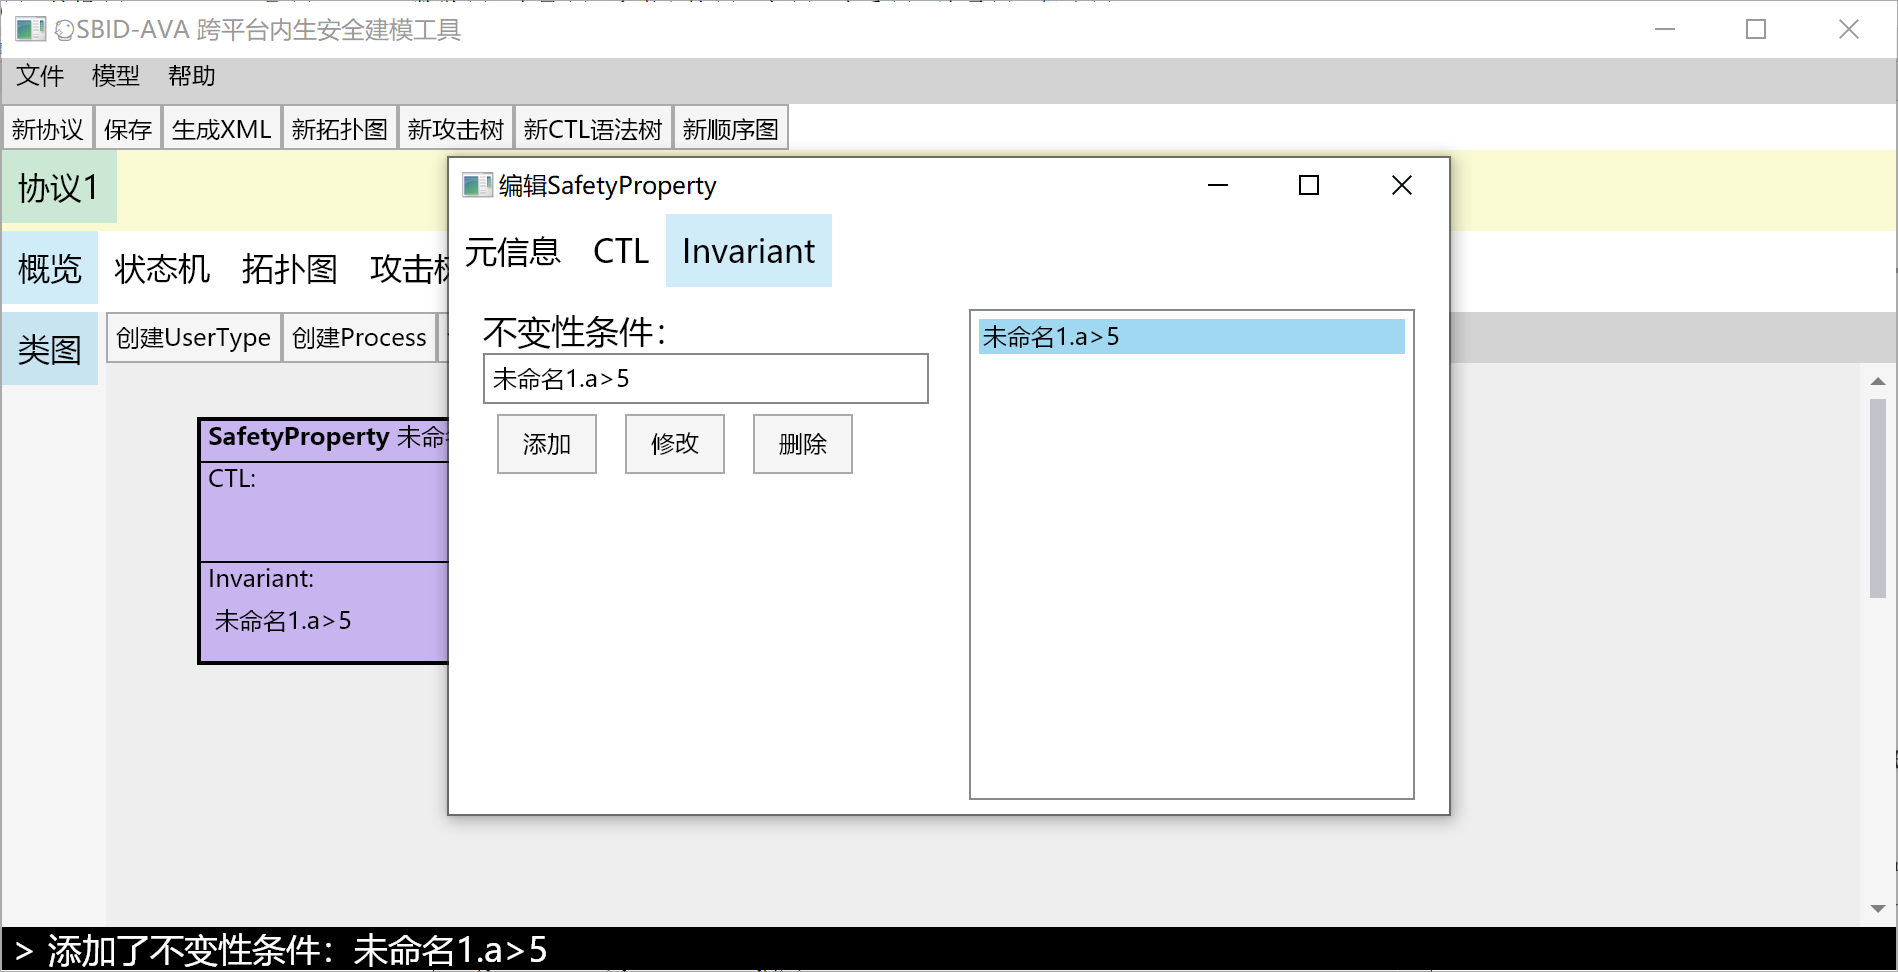
\includegraphics[width=12cm,height=6.75cm]{imgs/safety_edit_invariants.png}
	\caption{编辑Invariant}
	\label{safety_edit_invariants}
\end{figure}
\subsection{CTL公式}
\par
还可以用CTL公式定义功能安全性质。在Safety Property的编辑窗口,选择 [CTL]选项卡,可对CTL公式进行添加、修改和删除,如图\ref{safety_edit_ctl}所示。
\begin{figure}[h]
	\centering
	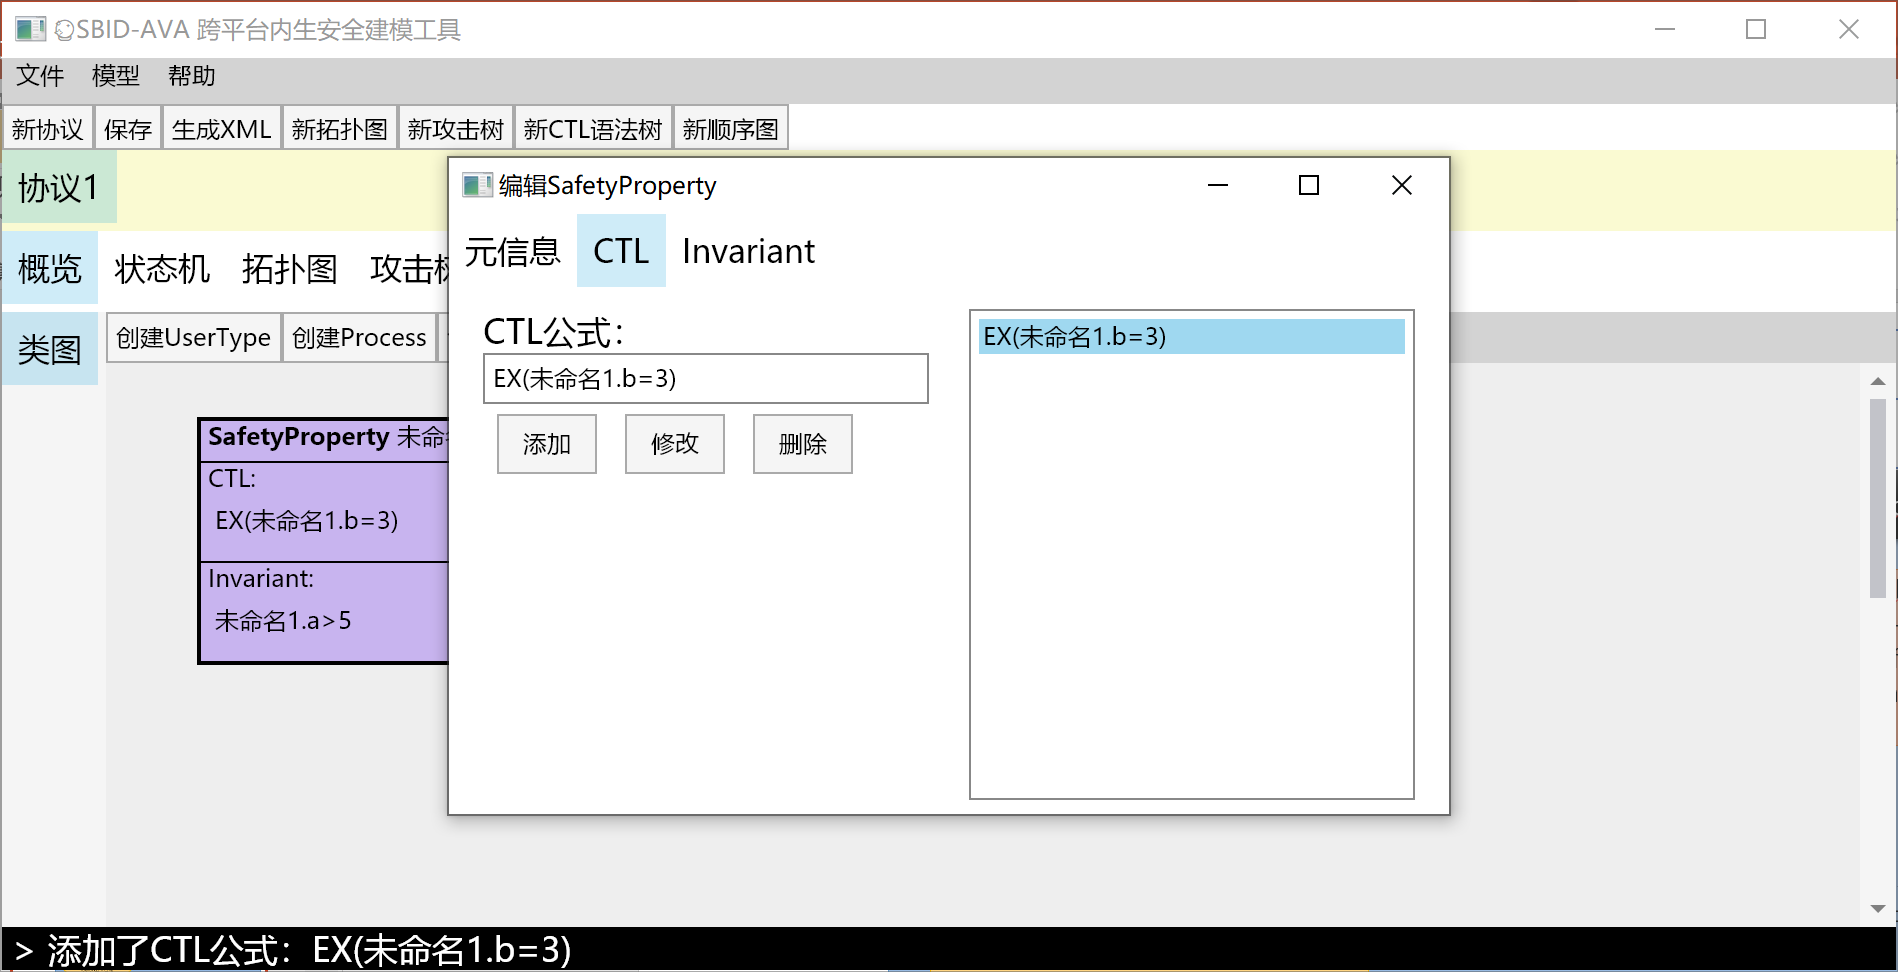
\includegraphics[width=12cm,height=6.75cm]{imgs/safety_edit_ctl.png}
	\caption{编辑CTL公式}
	\label{safety_edit_ctl}
\end{figure}

\section{Security Property}
Security Property描述了协议中进程模板涉及的信息安全性质,需要先定义好进程模板,再使用Security Property对其进行认证性和机密性的描述。在[协议>概览>类图]下,点击小工具栏上的[创建Security Property]按钮,即可创建新的Security Property的类图,如图\ref{create_security}所示。
\begin{figure}[h]
	\centering
	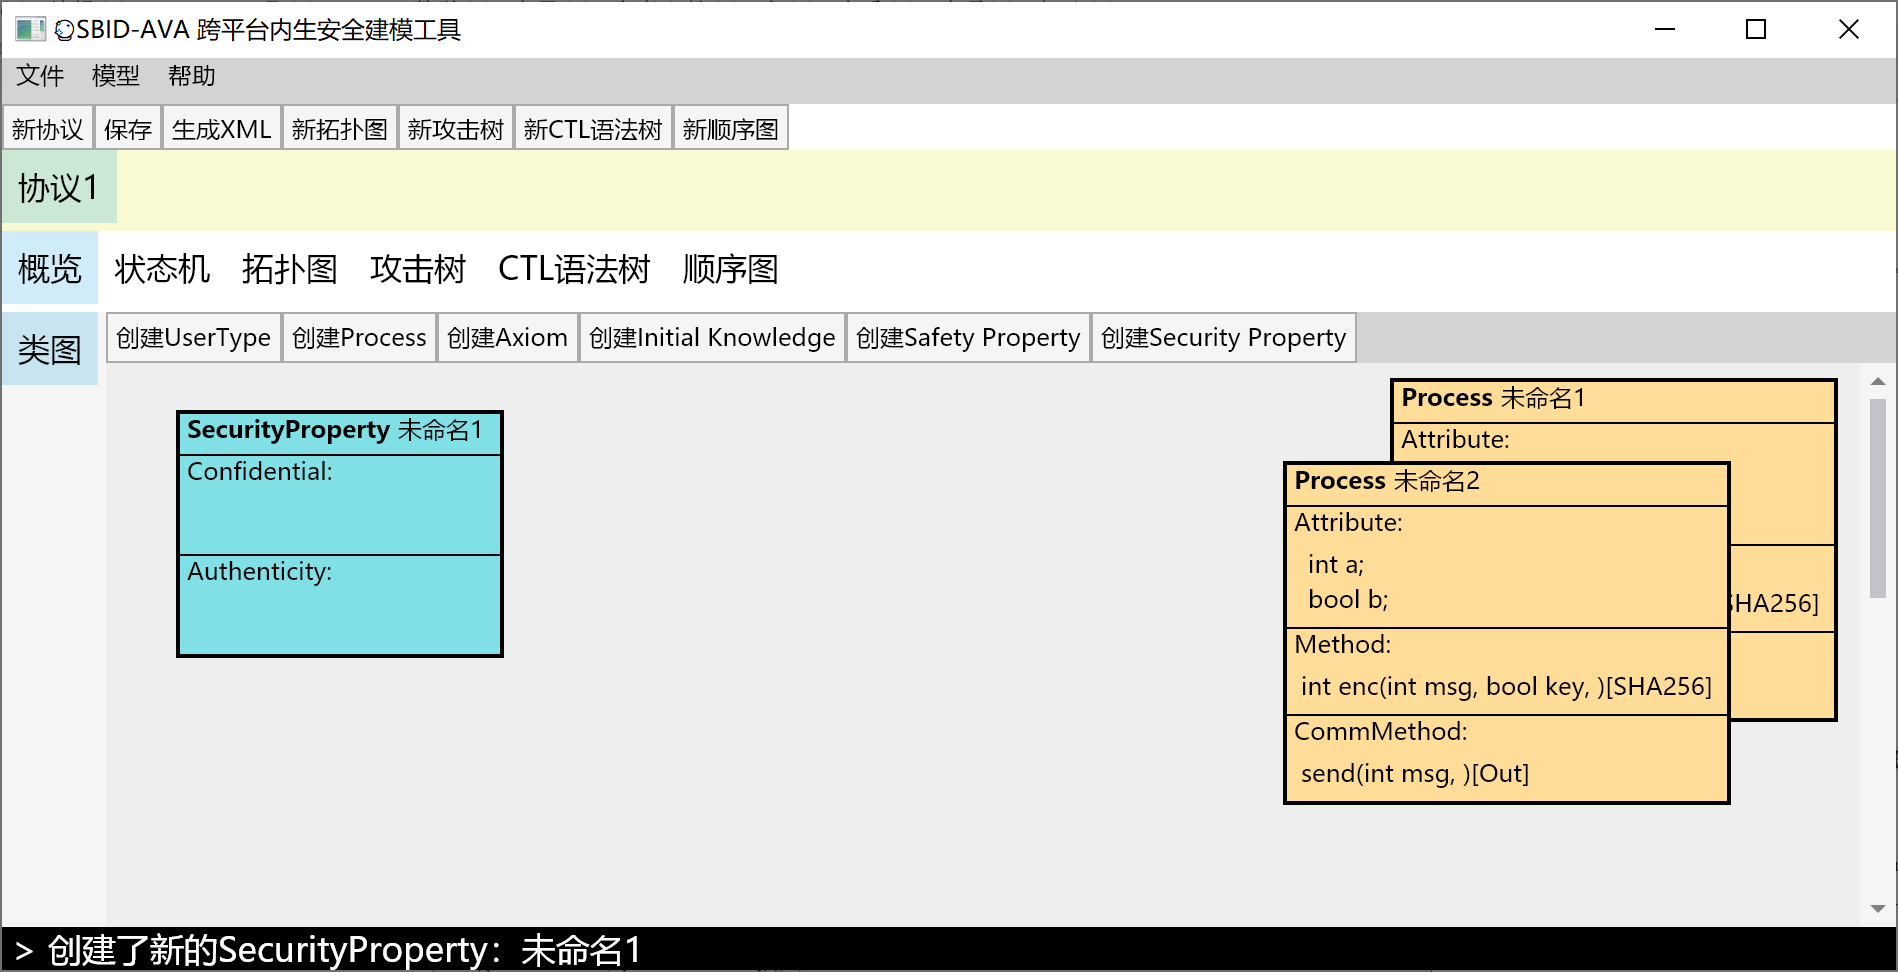
\includegraphics[width=12cm,height=6.75cm]{imgs/create_security.png}
	\caption{新创建的Security Property}
	\label{create_security}
\end{figure}
\par
在sbid工具中,支持用户对Confidential和Authenticity两类信息安全性质进行描述。
\par
在Security Property的类图上右键,呼出右键菜单,点击[编辑],即可打开在Security Property的编辑窗体。
\subsection{Confidential性质}
Security Property的Confidential用于定义进程属性的机密性,需要选中进程的某个属性。在Security Property的编辑窗口选择[Confidential]选项卡,可对Confidential进行添加、修改和删除,如图\ref{security_edit_confidential}所示。
\begin{figure}[h]
	\centering
	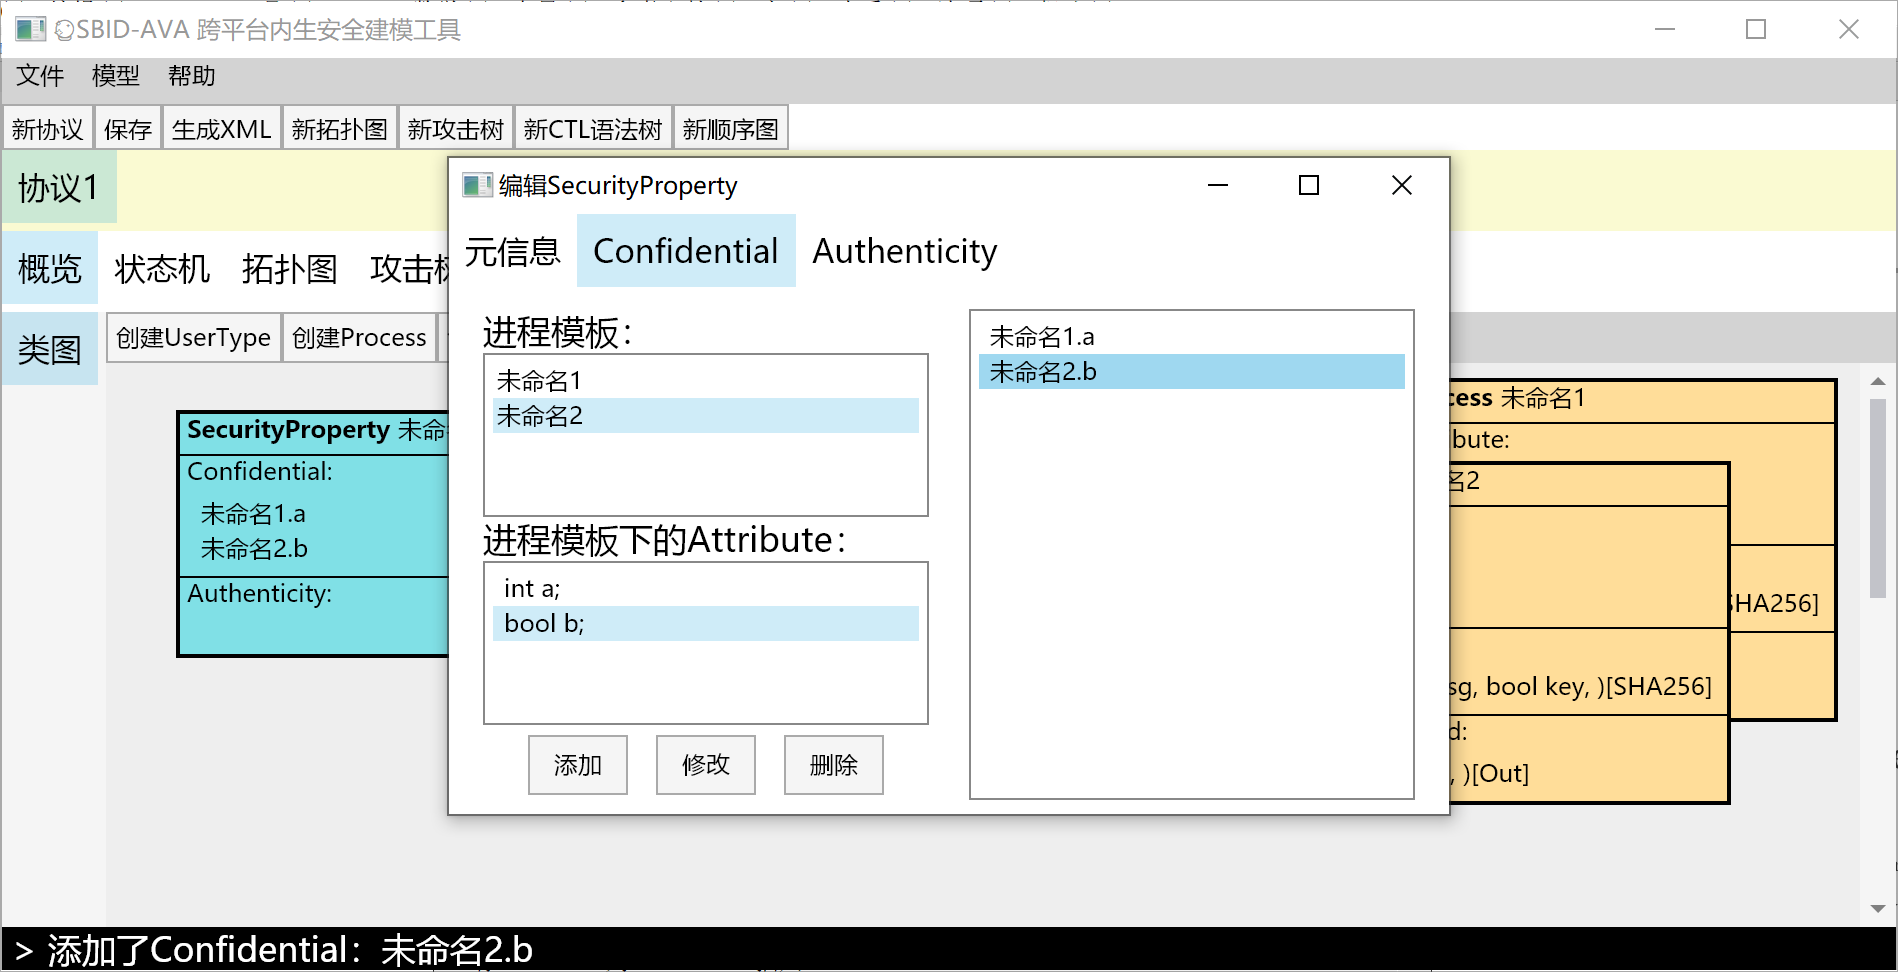
\includegraphics[width=12cm,height=6.75cm]{imgs/security_edit_confidential.png}
	\caption{编辑Confidential性质}
	\label{security_edit_confidential}
\end{figure}
\subsection{Authenticity性质}
Security Property的Authenticity用于定义进程状态中属性的认证性质,需要选中两对[进程,状态,属性]。在Security Property的编辑窗口选择 [Authenticity]选项卡,可对Authenticity性质进行添加、修改和删除,如图\ref{security_edit_authenticity}所示。
\begin{figure}[h]
	\centering
	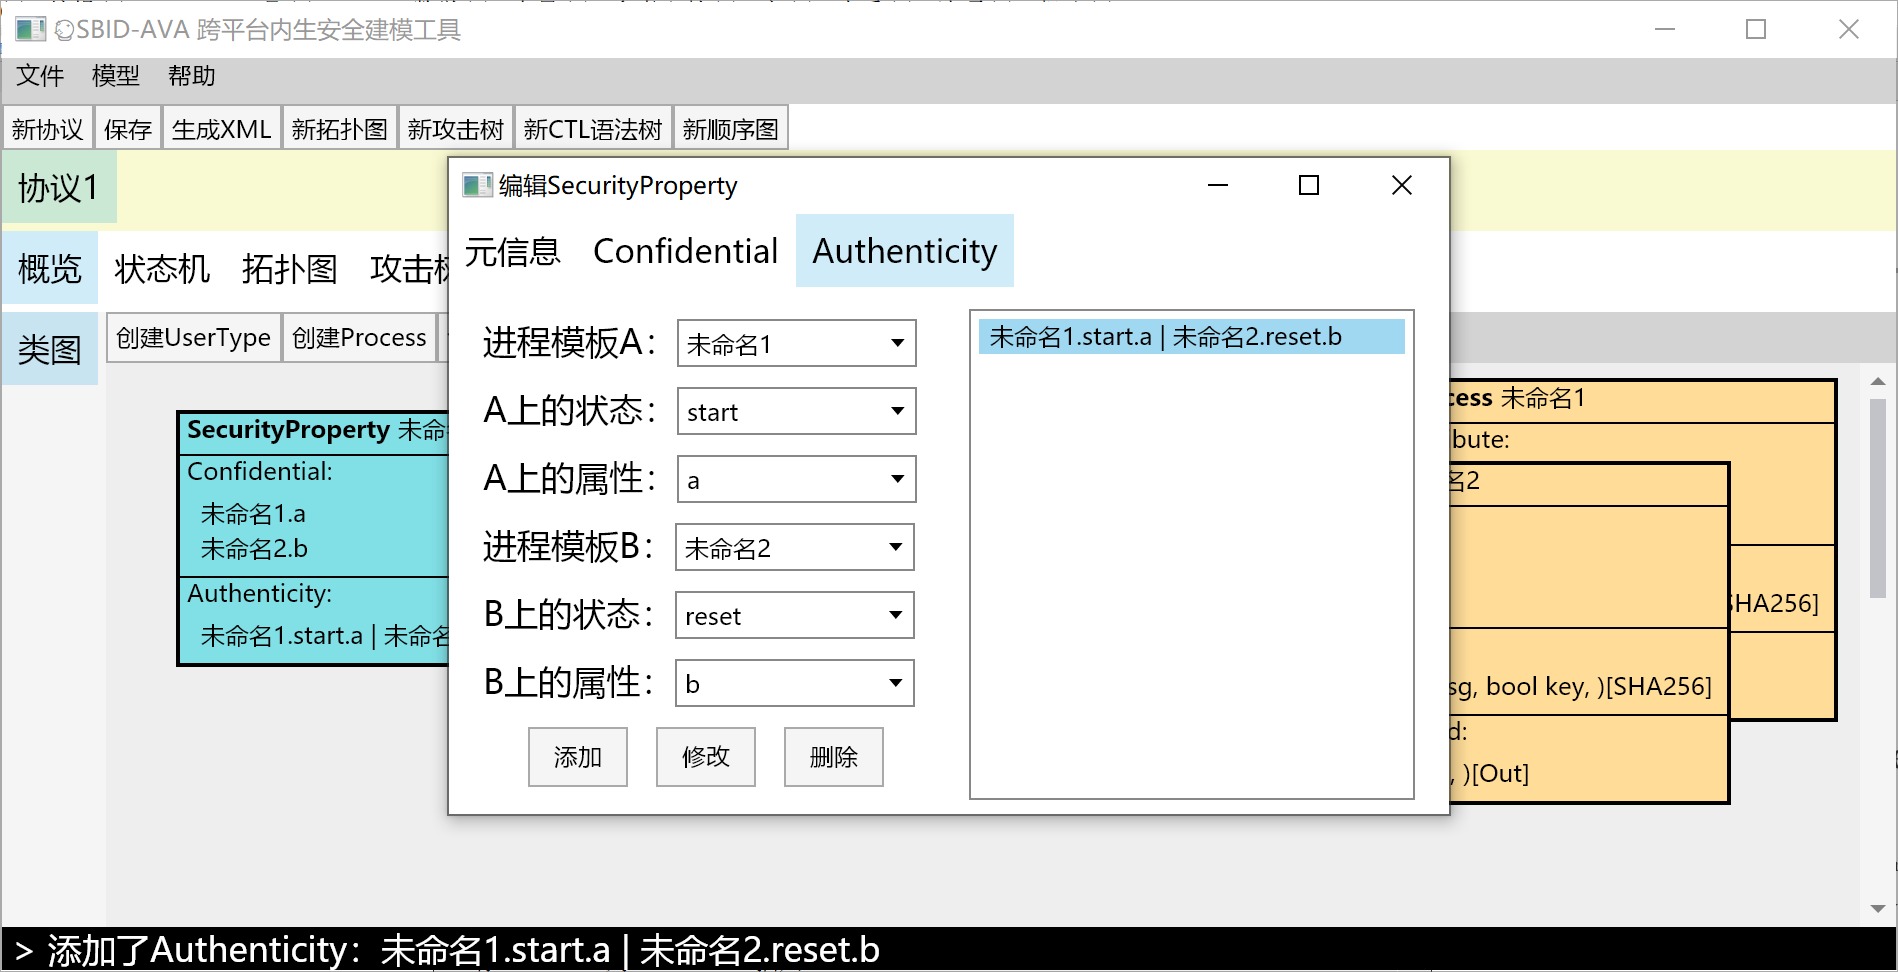
\includegraphics[width=12cm,height=6.75cm]{imgs/security_edit_authenticity.png}
	\caption{编辑Authenticity性质}
	\label{security_edit_authenticity}
\end{figure}
\par
需要注意,因为Authenticity性质需要使用进程模板状态机上的状态,所以对要使用的进程模板必须先定义好状态机,才能在Authenticity性质编辑时选中所需的状态。